%%
%%############################
\chapter{Fluid Tutorial: Flow around a Cylinder}
\label{tut_fluid:chap}
%Flow around a Cylinder - Von Karman vortex street

%%
%%============================
\section{Introduction}
In this tutorial we want to simulate the incompressible fluid flow around a cylinder.
For further details and references we refer the reader to:\\
W.A. Wall, PhD thesis, 1999
(available under \texttt{/lnm/literature/1999/})
\begin{figure}[h]
\begin{center}
 \includegraphics[scale=0.35]{pics/tut_fluid_problem}
 \caption{Problem definition and geometrical setup (with friendly permission ;-))}
\label{fig:tut_fluid_setup}
\end{center}
\end{figure}

%%
%%============================
\section{\baci{} Setup}

As science at the LNM doesn't focus on preprocessing, the 
research platform \baci{} is a solver only.
This means, you have to do the pre- and the postprocessing in a commercial
program (here: GID and Paraview). 
If you need more information on this software than provided here,
you can also refer to a special GID/Paraview tutorial, or - regarding
\baci{} - the LNM beginners guide.

The preprocessing software writes, after a successful input, a \emph{{*}.dat}
file containing all the information of the example (nodes, elements,
boundary conditions,..), which is then given to BACI for solving.

In order to use \baci{} for your special purposes (here: Fluid Flow), you have
to do a kind of setup first. This is done by changing the \texttt{defines.drt}
file in the \texttt{baci/config/} directory. 
First(!) make a copy of \texttt{defines.drt} in the same directory and name it \texttt{defines.drt.my}
Open your created working copy and select the
packages you need by uncommenting (i.e. removing the ``//`` in front) the according line. For all we do
here (and also for the third dimension) you will need the following,
so
\begin{itemize}
\item uncomment:
\begin{itemize}
\item Elements: D\_FLUID2, D\_FLUID3;
\item Additional features: BINIO;
\item Tools: RESULTTEST;
\item Fancy stuff: COLOROUTPUT, DSERROR\_DUMP;
\end{itemize}
\item Save the changes in the \emph{defines.drt.my} file. 
\item Next in the console the call (in the \baci{} directory) \emph{./configure
config/muench.fc6.ser config/defines.drt.my} creates the makefile needed
in the following steps. 
\item Use \emph{make clean} before recompiling. 
\item Next simply run \emph{make}.
\end{itemize}
This created everything necessary for BACI to solve your specific
problem.


%%
%%============================
\section{Preprocessing}

\subsection{Creating the Geometry}
Start GiD as described in the beginner's guide at section~\ref{beginner:sec:gid}.\\
If you use GiD for the first time, we recommend to do at least one of the tutorials
provided by GiD in order to get used to the basic geometry and mesh creation
tools available. You can access these tutorials via \textit{Help} $\rightarrow$ \textit{Tutorials}.
\\
Now you are ready to start:
\begin{enumerate}
\item \emph{Files $\rightarrow$ Save as} $\rightarrow$ \texttt{tut\_fluid.gid}
\item Draw a rectangle: \emph{{Geometry} $\rightarrow$ Create $\rightarrow$ Line}\\
\emph{Command} line: \texttt{-1,1}; \emph{Command}: \texttt{1,1}; \emph{Command}: \texttt{3,1}; \emph{Command}: \texttt{3,-1};  \emph{Command}: \texttt{1,-1}; \emph{Command}: \texttt{-1,-1};\emph{View
$\rightarrow$ Zoom $\rightarrow$ Frame} shows area of interest;
move $+$ pointer to your first point and click it; choose \emph{join}; hit
\texttt{ESC} to exit the line creation tool.
\item \emph{{Geometry} $\rightarrow$ Create $\rightarrow$ Line};
\emph{Command} line: \texttt{1,1}; choose \emph{join}; \emph{Command}: \texttt{1,-1}; choose \emph{join}; hit \texttt{ESC}.
% \item \emph{{Geometry} $\rightarrow$ Create $\rightarrow$ Object $\rightarrow$ Circle}\\
% \emph{Command} line: \texttt{0,0,0} (midpoint); choose \texttt{positive z} as normal vector and press \emph{Ok}; Command: \texttt{0.08} (for the radius);hit \texttt{ESC} to exit the circle creation tool;
% now delete the created circle surface by \emph{{Geometry} $\rightarrow$ Delete $\rightarrow$ Surface}; click on the surface (colored in magenta); hit \texttt{ESC}.
\item Some more lines are needed:\\
\emph{{Geometry} $\rightarrow$ Create $\rightarrow$ Line};
\emph{Command} line: \texttt{-1,1}; choose \emph{join}; \emph{Command}: \texttt{-0.05657,0.05657}; hit \texttt{ESC}.\\
\emph{{Geometry} $\rightarrow$ Create $\rightarrow$ Line};
\emph{Command} line: \texttt{1,1}; choose \emph{join}; \emph{Command}: \texttt{0.05657,0.05657}; hit \texttt{ESC}.\\
\emph{{Geometry} $\rightarrow$ Create $\rightarrow$ Line};
\emph{Command} line: \texttt{1,-1}; choose \emph{join}; \emph{Command}: \texttt{0.05657,-0.05657}; hit \texttt{ESC}.\\
\emph{{Geometry} $\rightarrow$ Create $\rightarrow$ Line};
\emph{Command} line: \texttt{-1,-1}; choose \emph{join}; \emph{Command}: \texttt{-0.05657,-0.05657}; hit \texttt{ESC}.

\item Now we create the four arcs forming the circle:\\ 
\emph{{Geometry} $\rightarrow$ Create $\rightarrow$ Arc};\\
select the point at coordinates (-0.05657,0.05657) with the mouse; choose \emph{join}; \emph{Command}: \texttt{0,0.08} (coordinates of second point); select the point at coordinates (0.05657,0.05657) as third point; choose \emph{join};\\
select the point at coordinates (0.05657,0.05657) with the mouse; choose \emph{join}; \emph{Command}: \texttt{0.08,0} (coordinates of second point); select the point at coordinates (0.05657,-0.05657) as third point; choose \emph{join};\\
select the point at coordinates (0.05657,-0.05657) with the mouse; choose \emph{join}; \emph{Command}: \texttt{0,-0.08} (coordinates of second point); select the point at coordinates (-0.05657,-0.05657) as third point; choose \emph{join};\\
select the point at coordinates (-0.05657,-0.05657) with the mouse; choose \emph{join}; \emph{Command}: \texttt{-0.08,0} (coordinates of second point); select the point at coordinates (-0.05657,0.05657) as third point; choose \emph{join};\\
finally, hit \texttt{ESC} to exit the arc creation tool.
\item Now we create the surfaces: \emph{{Geometry} $\rightarrow$ Create $\rightarrow$ NURBS Surface $\rightarrow$ Automatic}; enter number \texttt{4} and press \emph{Ok}. Six new surfaces are created (colored in magenta); now delete the created circle surface by \emph{{Geometry} $\rightarrow$ Delete $\rightarrow$ Surface}; click on the surface inside the circle to mark it; hit \texttt{ESC} to confirm.
\item Save the changes in your project: \emph{Files $\rightarrow$ Save}.
\end{enumerate}
After all this steps your geometry should look the same as depicted in figure \ref{fig:tut_fluid_geometry}.
\begin{figure}[h]
\begin{center}
 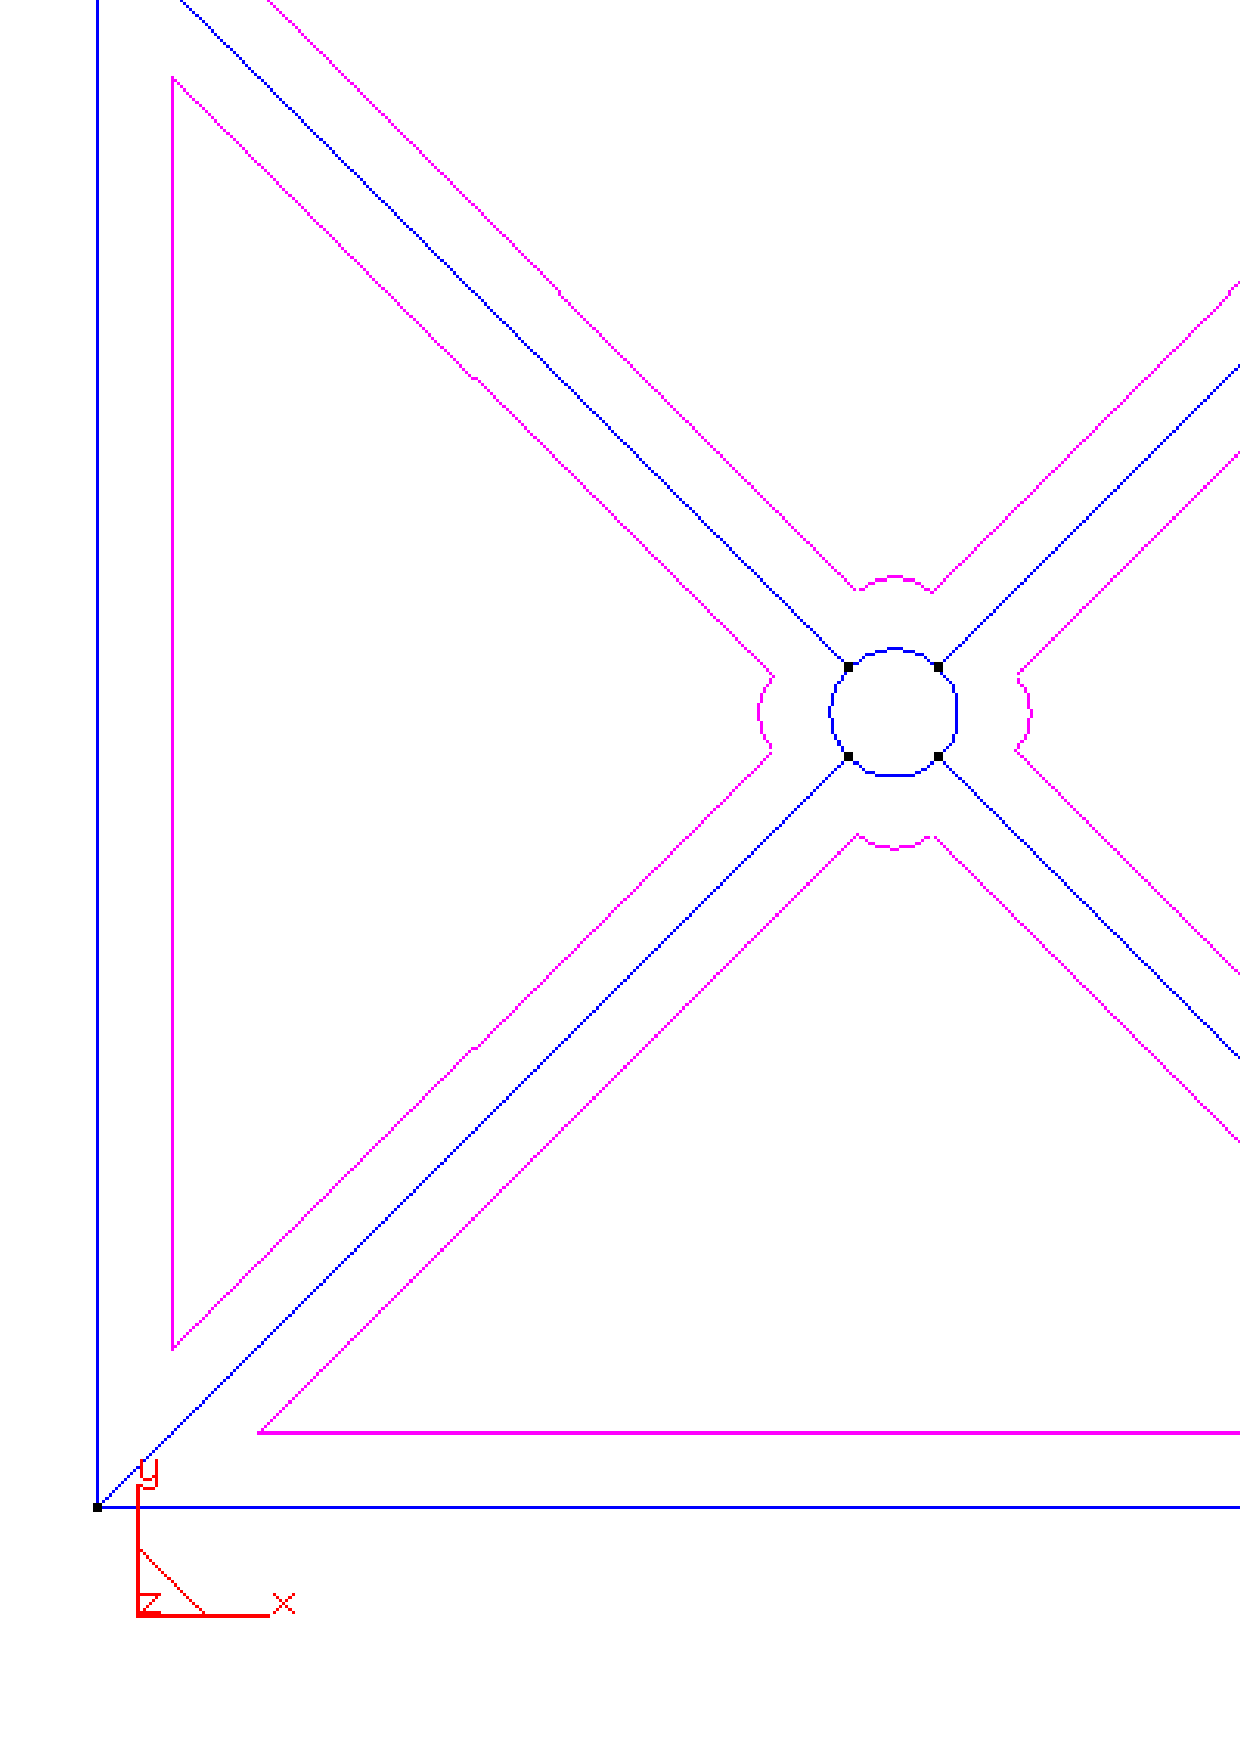
\includegraphics[scale=0.25]{pics/tut_fluid_geometry}
 \caption{Geometry created in GiD}
\label{fig:tut_fluid_geometry}
\end{center}
\end{figure}

\subsection{Show geometry labels (node-number, line-number, etc.)}
\label{tut_struct:sec:show-geo-label}

\begin{itemize}
\item \emph{View $\rightarrow$ Label $\rightarrow$ All} shows all geometry
labels/numbers 
\item \emph{View $\rightarrow$ Label $\rightarrow$ All in $\rightarrow$
node,line,...} shows selected geometry label 
\end{itemize}

\subsection{Using \emph{lnm\_general}}
\begin{enumerate}
\item Choose \emph{Data $\rightarrow$ Problemtypes $\rightarrow$ lnm\_general};
give \texttt{OK}
\item Apply boundary conditions (BCs): \emph{Data $\rightarrow$ Conditions
$\rightarrow$ SingleLayer}
\item In the \emph{SingleLayer} menu switch to \emph{line} (icon) and 
\texttt{\emph{L Dirich}}; 
tick \emph{2 on/off} to fixate the fluid velocity
to zero in $y$-direction; press \emph{Assign}; 
Select the two upper and the two lower horizontal lines; 
 then hit \texttt{ESC};\\
now set both \emph{1
on/off} and \emph{2 on/off} to \emph{on} to fixate the fluid velocity
to zero in $x$- and $y$-direction; press \emph{Assign}; 
Select the four arcs of the cylinder; 
 then hit \texttt{ESC};\\
now put a \texttt{1.0} in the field for \emph{value1} and change \emph{Load curve value1} from \emph{\texttt{none}} to \emph{\texttt{1}};
choose \emph{Assign}; select only the vertical line on the left hand side and hit
\texttt{ESC}; this line will act as inflow. 
\item Highlight the BCs: select \emph{Draw $\rightarrow$ colors} in the \emph{SingleLayer} window;
\emph{Finish}
\item It is good practice to explicitely specify BCs on those points, where two different BCs
come together. Since such a point belongs to more than one type of BC, you have to ensure what you want to have there.\\
In the \emph{SingleLayer} menu switch to \emph{point} (icon) and 
\texttt{\emph{P Dirich}} tick \emph{1
on/off} and \emph{2 on/off} to fixate the fluid velocity
to zero in $x$- and $y$-direction; press \emph{Assign}; 
Select the two points adjacent to the left vertical line; hit \texttt{ESC};
\item Setup time curve: select \emph{Data $\rightarrow$ Interval Data}; Select the tab named \emph{Curve1} and change \emph{Load Curve 1} to ; \emph{Typ curve 1} has to be set to \emph{\texttt{Explicit}}; hit \emph{Accept data} and then \emph{Close}.
\item Setup material: \emph{Data $\rightarrow$ Materials}; Select \texttt{\emph{MAT
fluid}}; insert for the (kinematic!)~\emph{viscosity} \texttt{0.004};
and for \emph{density} \texttt{1.0}; \emph{Assign $\rightarrow$
Surfaces}; Say \emph{Yes} when you are asked to save your data; now select all surfaces; \emph{Finish} or \texttt{ESC}; \emph{close} the material window. 
\item General problem data: \emph{Data $\rightarrow$ Problem Data $\rightarrow$
General Problem Data}; select tab \emph{General}; type in a \emph{Problem
title} \texttt{tut\_fluid}; \emph{Problem Type} \texttt{\emph{Fluid}};
Optimize maximal number of DOFs \emph{Max NumDOF} to \texttt{3}; \emph{Static/Dynamic}
to \texttt{\emph{Dynamic}};\emph{Linear Algebra} \texttt{\emph{Trilinos}}.
\item Include output: In \emph{General problem data} select tab \emph{IO}; tick \emph{OUTPUT BIN} and \emph{FLUID SOL}. 
\item More settings for dynamic case in \emph{Data $\rightarrow$ Problem
Data $\rightarrow$ Dynamic} in the tab \emph{Fluid}. For now, we just use the default preferencies.
Press \emph{Accept data} and then \emph{Close}.
\item Make geometric elements also design elements: execute \emph{ccarat Tools $\rightarrow$ Assign Design Numbers}\\
(Do NOT forget this step!)
\item Assign finite element: \emph{Data $\rightarrow$ Conditions $\rightarrow$
SingleLayer}; Tick \emph{Surfaces} (icon); Select \texttt{\emph{Fluid2}};
Keep all values as proposed; \emph{Assign} the Fluid2 element to all surfaces; hit \texttt{ESC}.
\item Prepare the structured mesh: \emph{Meshing $\rightarrow$ Structured
$\rightarrow$ Surfaces}; Select all surfaces; \texttt{ESC}; dialogue
\emph{Enter number of cells to assign to lines}:\\
enter \texttt{37}; give \emph{OK}; now select the horizontal line of the right surface (opposite
lines get selected automatically); \texttt{ESC};\\
enter \texttt{34}; give \emph{OK}; Select the very right vertical line; \texttt{ESC};\\ 
enter \texttt{30}; give \emph{OK}; Select the upper and lower horizontal lines on the left part of the geometry; \texttt{ESC};\\
enter \texttt{22}; give \emph{OK}; Select the very left vertical line; \texttt{ESC};\\
enter \texttt{52}; give \emph{OK}; Select all four diagonal lines; \texttt{ESC};\\
finish with \emph{Cancel}.
\item Generate the mesh: \emph{Meshing $\rightarrow$ Generate...};
Ignore proposed element size and give \emph{OK}; see generated mesh;
you can toggle between mesh and geometry by going to \emph{Meshing
$\rightarrow$ Mesh view}.
\item We want to improve our structured mesh around the cylinder:
\emph{Meshing $\rightarrow$ Structured $\rightarrow$ Concentrate elements};
select the four diagonal lines; hit \texttt{ESC}; 
\emph{Start Weight} is \texttt{0.0} and \emph{End Weight} is \texttt{0.1};
select \emph{Ok} and press \texttt{ESC}.
\item Generate the mesh again: \emph{Meshing $\rightarrow$ Generate...}; compare the resulting mesh with figure \ref{fig:tut_fluid_mesh}.
\item Finally create the \baci{} input file: \emph{Calculate $\rightarrow$ Calculate};
this should produce \texttt{\emph{tut\_fluid.dat}}.
\end{enumerate}
%
\begin{figure}[h]
\begin{center}
 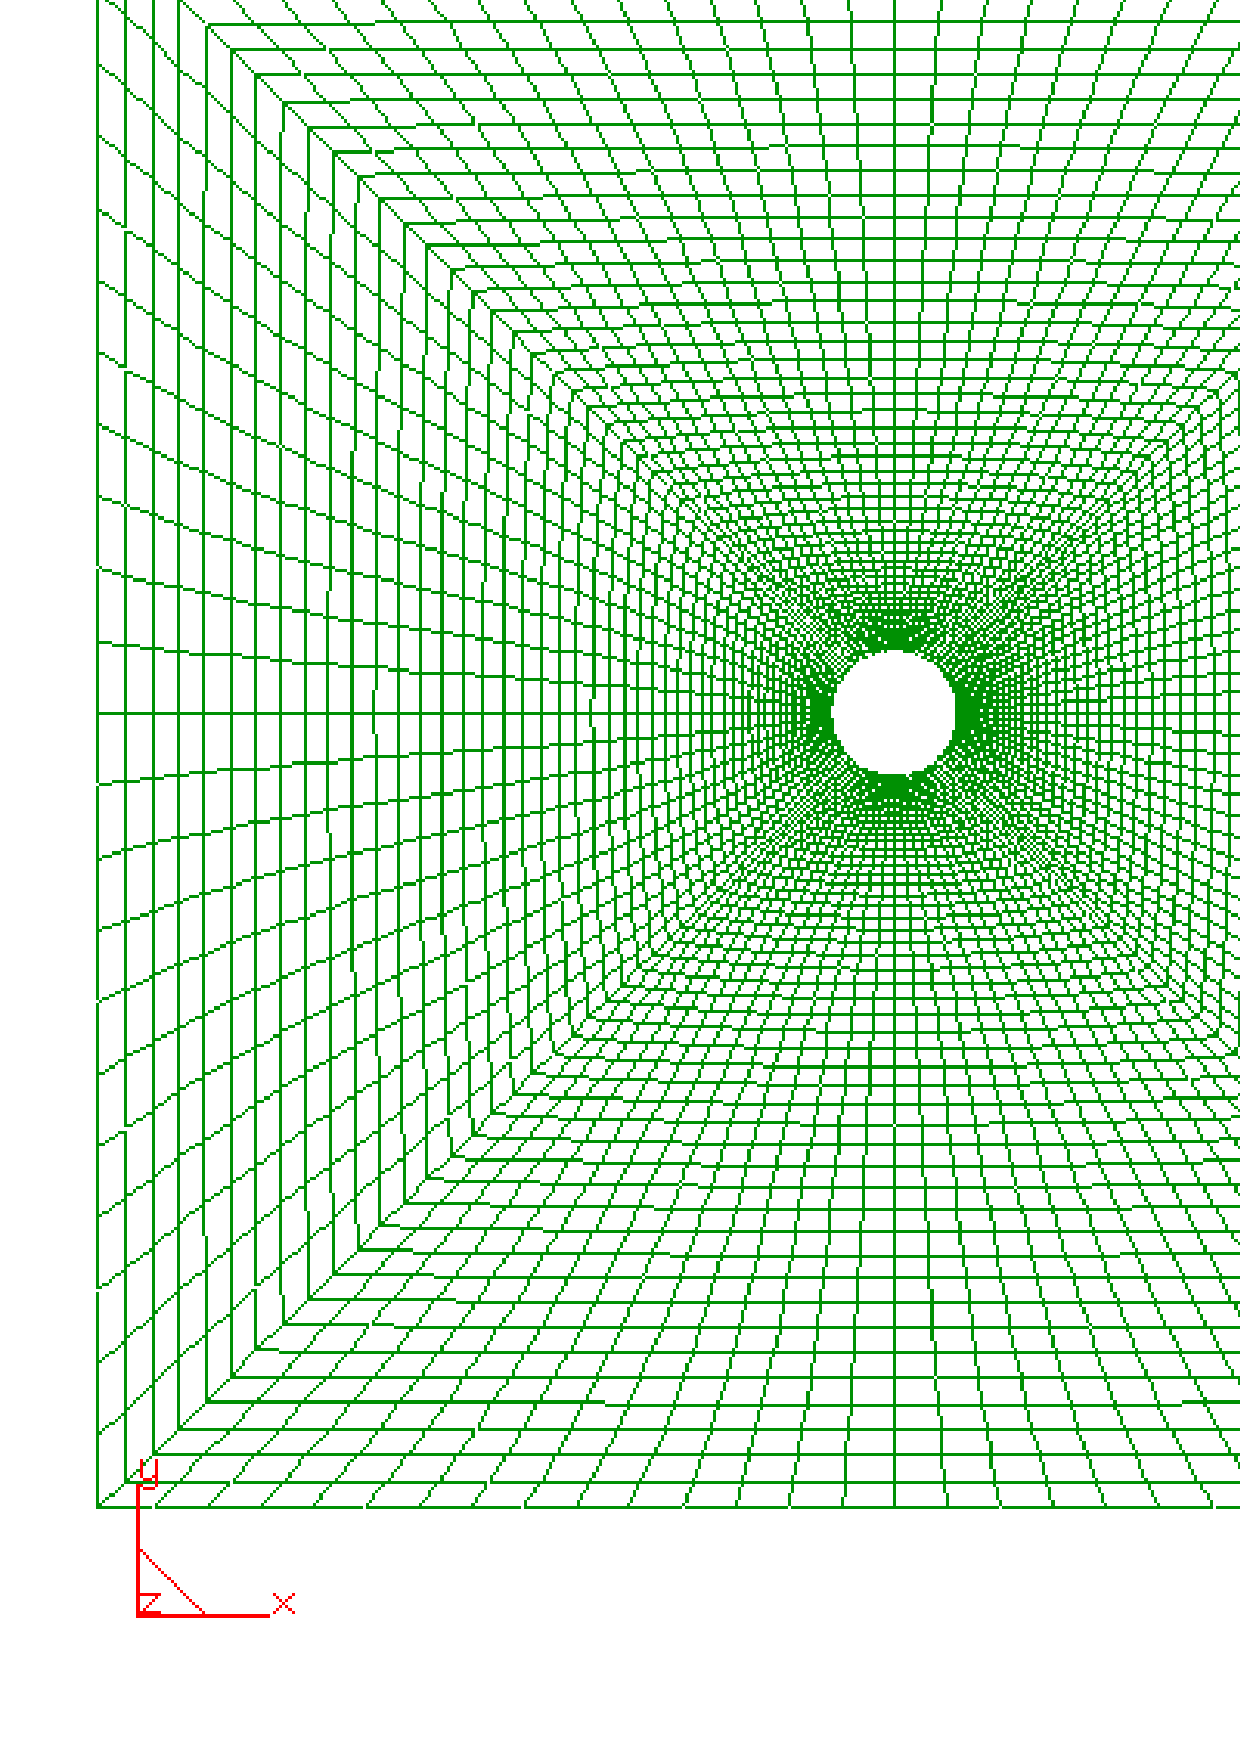
\includegraphics[scale=0.25]{pics/tut_fluid_mesh}
 \caption{Structured mesh created with GiD}
\label{fig:tut_fluid_mesh}
\end{center}
\end{figure}
%%
%%============================
\section{Solving the problem with \baci{}}

After the successful creation of the input file in the previous section,
you are ready to start the simulation with \\
\texttt{./cca\_fc6\_ser.fast tut\_fluid.dat outputname}
%%
%%============================
\section{Postprocessing}

For the postprocessing we want to use a software called \emph{paraview}. 
In principal you can use GID (or any other supported tool) for visualization 
of your data as well.

\subsection{Filtering result data}
\begin{itemize}
\item Before you can admire your results, you have to generate a filter 
which converts the generic binary \baci{} output to the desired format.
Starting from the \baci{} directory execute \texttt{make post\_drt\_ensight}.
\item The filter should now be available in your \baci{} directory. Filter your results with
the call (inside the \baci{} directory): \texttt{post\_drt\_ensight -\,-file=outputname} 
\item Further options of the filter program are made visible by the command \texttt{post\_drt\_ensight}.
\end{itemize}

\subsection{Visualize your results in Paraview}
\begin{itemize}
\item After the filtering process is finished open \emph{paraview} by typing \newline
\texttt{/lnm/programs/paraview-3.0.2-Linux-x86/bin/paraview \&}
\item \emph{File$\to$Open} and select the filtered \emph{*.case}
file: \emph{outputname.case}
\item shift \emph{Byte order} to \emph{little endian}. 
\item press \emph{Accept} to activate the display.
\item choose time step 100 in the top menu bar 
\item in the \emph{Display} tab (section \emph{Color}) press \emph{Rescale to Data Range}. At \emph{Color by} you can choose now
between \emph{Point pressure} and \emph{Point velocity}, whatever
you want to display.
\item For the scale, press \emph{Edit Color Map}, choose the tab \emph{Color legend} and activate \emph{Show color legend}.
\end{itemize}
\begin{figure}[h]
\begin{center}
 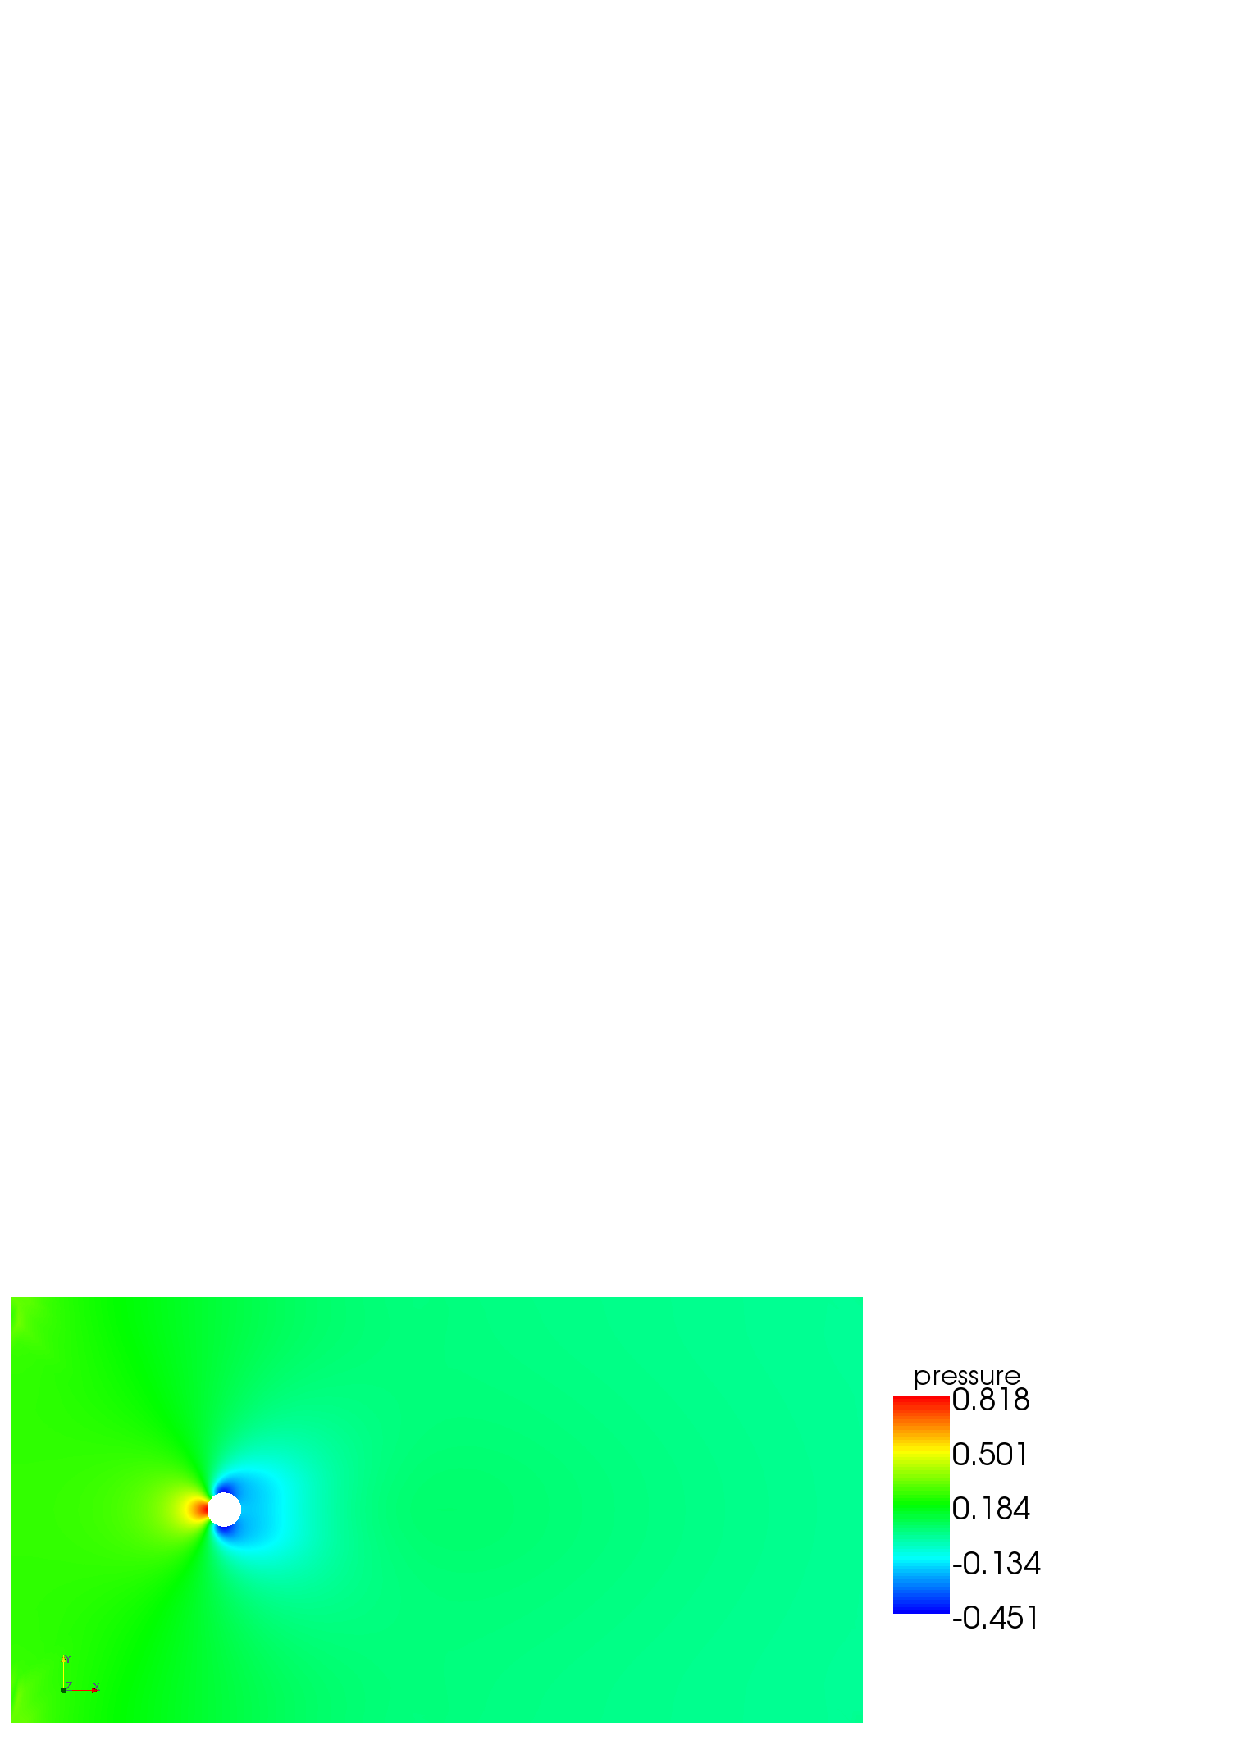
\includegraphics[scale=0.7]{pics/tut_fluid_pres}
 \caption{pressure distribution at time step 100}
\label{fig:tut_fluid_mesh}
\end{center}
\end{figure}
